\chapter{Der Money-Coutts-Prozess}

\citet{EMT1974} beschreiben einen Prozess zur iterativen Erzeugung von Kreisen in einem Dreieck.
Zunächst wird ein Kreis eine Ecke des Dreiecks gezeichnet --
er berührt die beiden Seiten, die diese Ecke bilden.
Dann werden reihum weitere Kreise in die Ecken gezeichnet,
sie zusätzlich den jeweils vorher gezeichneten Kreis berühren.

Der Mittelpunkt eines solchen Kreises liegt dabei immer auf der Winkelhalbierenden des Winkels der Ecke, in die der Kreis positioniert wird.
Kennt man den Radius des zu positionierenden Kreises, so ist die Position des Mittelpunktes eindeutig.
Bildhaft schiebt man den Mittelpunkt des Kreises entlang der Winkelhalbierenden so nah an die Ecke des des Polygons,
dass der Kreis die beiden anliegenden Seiten der Ecke berührt.

Die Untersuchung dieses Prozesses lieferte das Ergebnis,
dass der Money-Coutts-Prozess 6-periodisch ist,
also der siebte gezeichnete Kreis mit dem initial gezeichneten übereinstimmt.
Ein Beweis wird \Cref{six-circle-theorem} geführt.

\citet{Taba2013} merken dazu an,
dass das von \citet{EMT1974} definierte Vorgehen weiter spezifiziert werden sollte.
So kann es passieren, dass große Kreise nicht die beide Seiten berühren,
sondern nur die Verlängerungen dieser.
Im Prozess gibt es Wahlmöglichkeiten.
Der neue Kreis kann aus Sicht der Ecke vor oder hinter seinen Vorgänger gezeichnet werden.
% TODO: Anmerkungen zum MCP: Wahl hier schon betrachten?

Die vorliegende Arbeit betrachtet die Erweiterung des Money-Coutts-Prozesses auf Polygone.
Es werden folgende Konventionen zur Notation verwendet:
Im gegebenen Polygon $P$ mit Ecken $A_1$ bis $A_n$ sei $a_i$ die Länge der Seite zwischen den Ecken $A_i$ und $A_{i+1}$.
Die Größe des Winkels in der Ecke bei $A_i$ beträgt $2\alpha_i$.
Das Winkelmaß $\alpha_i$ ist also gerade die Hälfte des Innenwinkels bei $A_i$.

\begin{figure}[htbp]
    \begin{tikzpicture}
    \draw
    (3,0) coordinate (a) node[right] {a}
    -- (0,0) coordinate (b) node[left] {$A_1$}
    -- (2,2) coordinate (c) node[above right] {c};
    % \draw pic["$\alpha_1$", draw=orange, <->, angle eccentricity=1.2, angle radius=1cm]{angle=a--b--c};

\end{tikzpicture}
    \caption{Darstellung der Notationen}
\end{figure}

\paragraph{Konstruktion im Money-Coutts-Prozess}

Zwei Kreise, die nacheinander erzeugt werden, berühren beide die Kante $a_i$.
Konstruiert man ein rechtwinkliges Dreieck wie in \Cref{fig:mcp:two-circles},
ergibt sich mit dem Satz des Pythagoras folgender Zusammenhang:
\begin{equation}
    a_i = r_i\cot\alpha_i + 2\sqrt{r_i r_{i+1}} +r_{i+1}\cot\alpha_{i+1}
    \label{mcp:two-circles}
\end{equation}

\citet{Taba2000} führt nun neue Variablen ein, die \citet{Troub2000} \emph{Tabachnikov-Koordinaten} nennt:

\begin{equation}
    \begin{array}{ccc}
        c_i = \sqrt{a_i}, & u_i = \sqrt{r_i \cot\alpha_i}, & e_i = \sqrt{\tan\alpha_i \tan\alpha_{i+1}}
    \end{array}
    \label{mcp:taba-coordinates}
\end{equation}

Durch Verwendung dieser Koordinaten erhält man aus \Cref{mcp:two-circles}:
\begin{equation}
    c_i^2 = u_i^2 + 2 e_i u_i u_{i+1} + u_{i+1}^2
    % TODO: ist diese Umformung wichtig?
    = u_i (u_i + e_i u_{i+1}) +u_{i+1} (u_{i+1} + e_i u_i)
\end{equation}

% siehe https://www.wolframalpha.com/input?i=+u%5E2+%2B+2+e+u+v+%2B+v%5E2+%3D+c%5E2
Diese in $u_{i+1}$ quadratische Gleichung wird weiterhin nach $u_{i+1}$ aufgelöst:
\begin{equation*}
    u_{i+1} = - e_i u_i \pm \sqrt{c_i^2 + (e_i^2 - 1) u_i^2}
\end{equation*}
% TODO: ist e_i > 1?
% TODO: wo kommen die Beträge her?
% TODO: welches nehmen wir von \pm ?
% TODO: kleinere Lösung wählen für den kleineren Kreis?

\begin{equation}
    u_{i+1} = \text{\% TODO}
    \label{mcp:iteration-equation}
\end{equation}

\begin{figure}[htbp]
    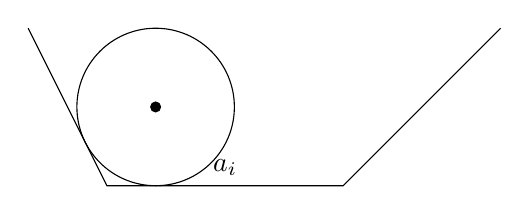
\begin{tikzpicture}
    % TODO: finish this
    \draw (0,2) -- (1,0) coordinate (a)
    -- (4,0) coordinate (b)
    -- (6,2);
    \draw (2.5,0) node[anchor=south] {$a_i$};
    % is this the golden ratio?
    \draw (1.618,1) circle (1cm);
    \fill (1.618,1) circle (2pt);
\end{tikzpicture}
    \caption{Zwei aufeinander folgende Kreise im Money-Coutts-Prozess.}
    \label{fig:mcp:two-circles}
\end{figure}


